\chapter{Background}
\label{chap:background}

The topic of this work evolved from the situation that the healthcare robotic applications of the University of Auckland should be equipped with mechanisms for ensuring safety.
The motivation for it is described in section~\ref{sec:healthbotapplication} as well as the robots used, the kind of applications running on them, and their technical background.

The visual programming environment used for the programming of these robots is presented in section~\ref{sec:robostudio}.
For the understanding of safety concepts which this work is based on, a short introduction about functional safety is given in section~\ref{sec:behaviourchecking}. In section~\ref{sec:relatedwork} other work and programs related to this work are examined.




\section{Healthbot application}
\label{sec:healthbotapplication}

%\begin{wrapfigure}{r}{0.38\textwidth}
%  \centering
%  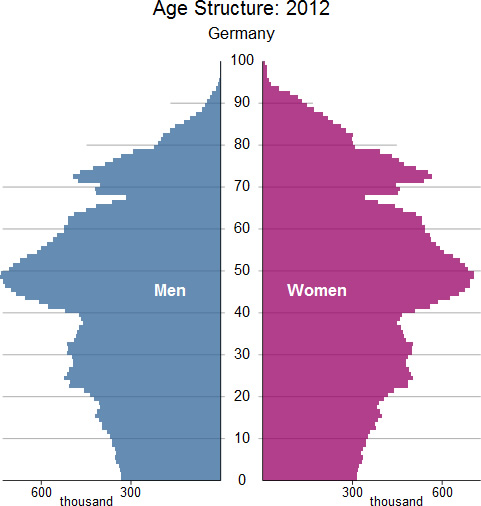
\includegraphics[width=0.34\textwidth]{populationpyramide}
%  \caption{Age structure.}%Population pyramide of germany.}
%  \label{fig:populationpyramide}
%\end{wrapfigure}
In some countries, among New Zealand and Germany, the average age of population is constantly increasing. Owing to excellent achievements in medicine as well as higher living standards, humans can enjoy longer lifes. Also decreasing birth rates contribute to an upward drift of the dominating age range. As a result, the industrial sectors of professional health care and social institutions are required more than ever.
However, a strong deficit of professionals is denoted in the healthcare branch and availability is far behind demand. One reason for this might be below average low salaries for employees in the healthcare sector. But, just raising the salary isn't leading to the desired results since the majority of the older people can't even afford a nurse to today's prices.

Aiming for fillig the constantly increasing gap in professional personnel for healthcare of the elderly and bypassing the financial burden, service robots are supposed to more and more undertake the task of care.
There are lots of possible tasks a robot could do such as taking the blood pressure, guiding medication intake, detecting falls or just entertaining with music, video or internet.
This challenge as a goal, the healthcare robotics team at the University of Auckland researches this topic and builds service robots for supporting the elderly in their daily life.

The two newest robots IrobiQ and Cafero are shown in figure~\ref{fig:irobiq_cafero}.
These mobile 
\begin{wrapfigure}{r}{0.60\textwidth}
  \centering
  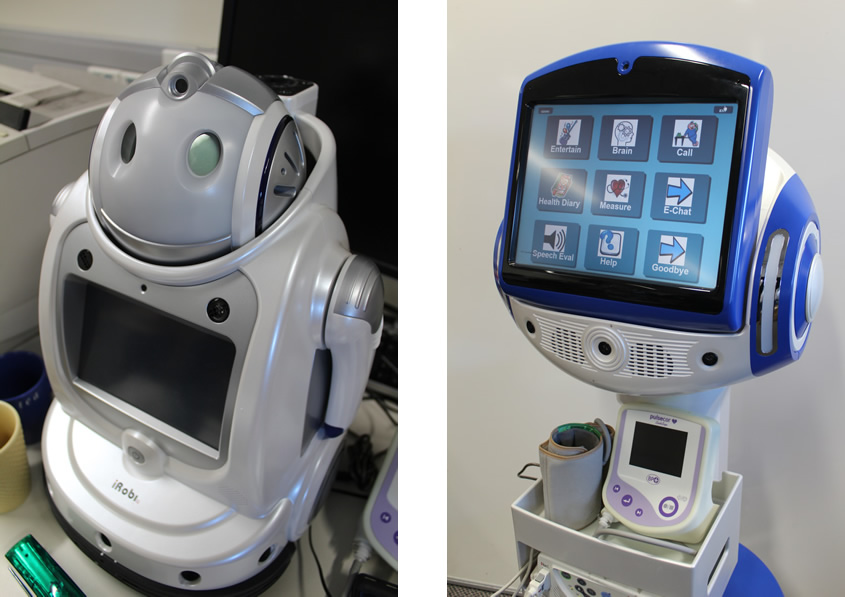
\includegraphics[width=0.56\textwidth]{irobiq_cafero}
  \caption{IrobiQ and Cafero, two robots of the healtcare project.}
  \label{fig:irobiq_cafero}
\end{wrapfigure}
robots are equipped with a touch display for presenting screens and receiving user input. Furthermore, they are equipped with additional external tools such as the blood pressure measurement device.
Applications running on the robot use the touch display to present screen dialogs to the user and use speech synthesis in order to give also accoustic feedback. User inputs or response from devices cause dialogs to change. Figure~\ref{fig:screenflow_example} presents a small example of such a screen-flow based application, which uses response from a camera and user input for navigating through the screen-flow.

%, and they can access devices such as the camera for face recognition or the blood pressure measurement tool. 

There is a program interpreter running on the robots which can load and execute program files. Screen dialogs get generated and displayed on the touch screen.
%This makes the program behaviour replaceable and maintenance can be done easily.
The interpreter processes programs written in Robot Behaviour Description Language (RBDL), a domain specific language (DSL) based on XML, which has been developed particularly for the healthcare robotics applications. It allows defining state machine based program behaviour and creating UI elements for screen visualizations. An example implementation of one state in RBDL is shown in listing~\ref{lst:RBDL}.

\begin{figure}[htbp]
  \centering
  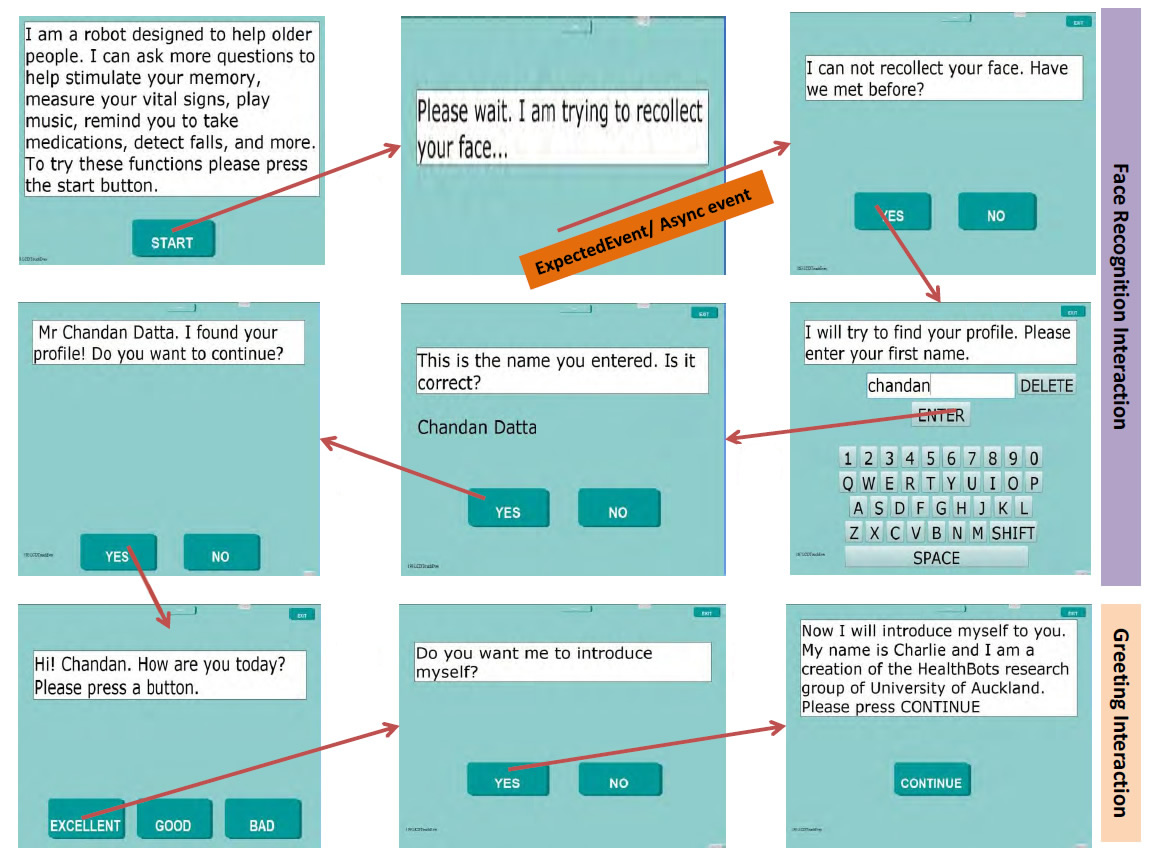
\includegraphics[width=\linewidth]{screenflow_example} 
  \caption{Robot screen-flow dialog based interaction example~\cite{robostudio}.}
  \label{fig:screenflow_example}
\end{figure}

\lstset{
  basicstyle=\ttfamily,
  columns=fullflexible,
  showstringspaces=false,
  commentstyle=\color{gray}\upshape
}

\lstdefinelanguage{XML}
{
  morestring=[b]",
  morestring=[s]{>}{<},
  morecomment=[s]{<?}{?>},
  stringstyle=\color{black},
  identifierstyle=\color{darkblue},
  keywordstyle=\color{cyan},
	morekeywords={%no, type_, senderid, receiverid, name_, vartype, label, width, height, x, y, textsize, preconditions
	}
}

\begin{lstlisting}[float = htbp, language=XML, captionpos=b, breaklines=true, showspaces=false, showtabs=false, tabsize=2, caption=Example of a state defined by RBDL~\cite{robostudio}., label=lst:RBDL]
<state no="84">
	<backgroundactions>
		<rocosmessage type="EVENT MESSAGE" senderid="RCP" receiverid="NA" name="FDSessionStart">
			<parameter vartype="text" type="unsigned int" name="id">1</parameter>
			<parameter type="string" name="" />
		</rocosmessage>
	</backgroundactions>
	<screen>
		<components>
			<button label="START" width="250" height="100" x="387" y="600" textsize="40">
				<event name="clicked">
					<action preconditions="no" name="transition">
						<parameter>
							<type>state</type>
							<name>n</name>
							<value>86</value>
						</parameter>
					</action>
				</event>
			</button>
		</components>
	</screen>
	<expectedevents>
		<event name="TimeOut">
			<action preconditions="no" name="transition">
				<parameter>
					<type>state</type>
					<name>n</name>
					<value>VARFirstScreen</value>
				</parameter>
			</action>
		</event>
	</expectedevents>
</state>
\end{lstlisting}

For each state of the program, background actions can be defined. They are transparent to the user and run in background. Text messages can be sent or external devices can be acessed, for example. The latter is realized with web services~\cite{webservices} to obtain a modular design.
Some states can also have screen definitions with buttons, messages, videos, etc., on it. These are displayed to the user when the respective state is active. Once displayed, buttons can be clicked and trigger events.
The behaviour of events can be mapped in the expectedevents tag. It lists all events which are processable by the current state and defines the corresponding behaviour such as triggering transitions to other states.

For this work the most important thing about the RBDL to remember is that it can define state machine behaviour with states, transitions and events. This fact was the basis for later decisions regarding used safety mechanisms.



%Zugriff auf devices via web services
%Windows is used as operating system on the robots and the programs are executed in Adobe flash and Actionscript. External devices are accessed over web




\section{Robostudio}
\label{sec:robostudio}

In the beginning all programming of the robot behaviour was done by directly editing the XML code mentioned in the previous section by using a text editor. But huge code files and occasional code edits made further maintenance and change requests difficult up to impossible to realise. For this reason, Chandan Datta, PhD student at the University of Auckland, developed a visual programming environment for developing robot behaviour on top of RBDL: Robostudio~\cite{robostudio} allows to easily edit the program behaviour on a visual layer and generates the corresponding program file containing the RBDL code fully automatically. This file can be downloaded to the robot and executed by the interpreter. Figure~\ref{fig:robostudio_proceeding} illustrates the steps of robot behaviour development.

\begin{figure}[htbp]
  \centering
  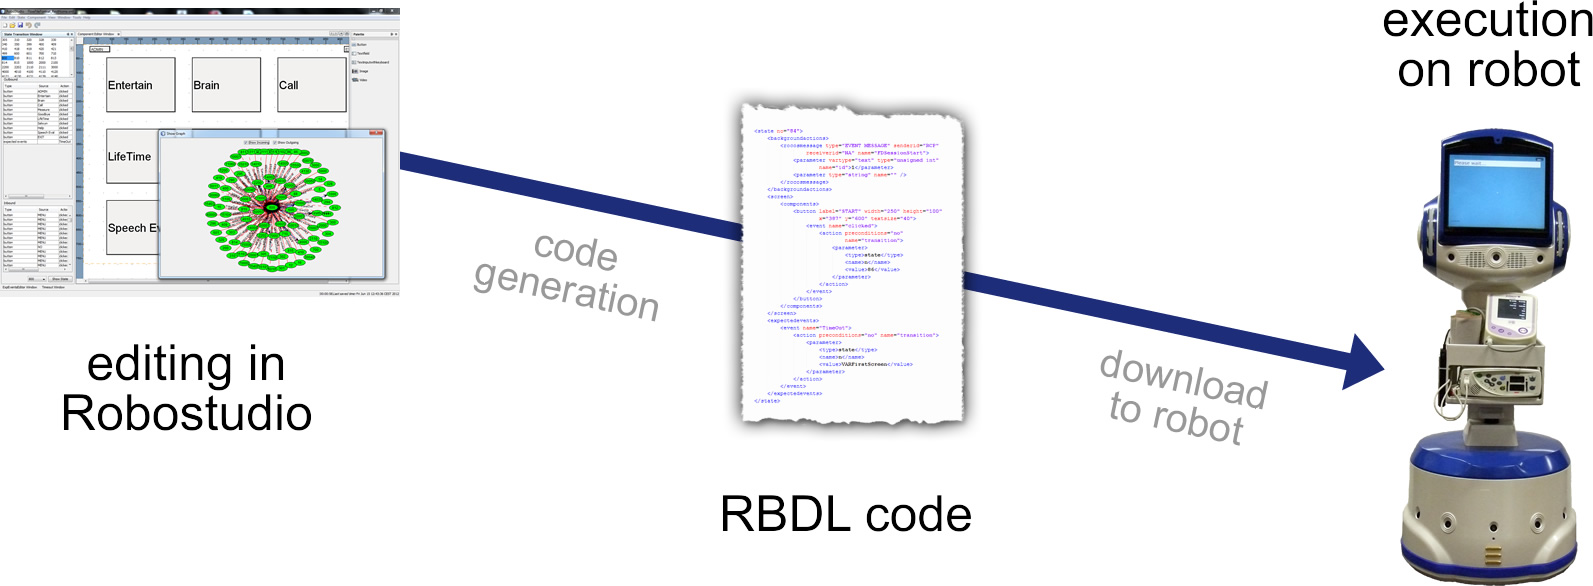
\includegraphics[width=\linewidth]{robostudio_proceeding} 
  \caption{How Robostudio is used for robot behaviour development.}
  \label{fig:robostudio_proceeding}
\end{figure}

Robostudio is an editor fully written in Java and implemented as a NetBeans rich client application.
Several windows and views provide visual tools for editing and understanding robot behaviour as well as screen dialog design. As depicted in figure~\ref{fig:robostudio_vpe}, the editor integrates a \emph{State Navigator Window} (1) in the top left corner where all existing states are listed. Below an overview about all incoming and outgoing transitions is given. New states can be created and existing states can be deleted. A click on one particular state id in the \emph{State Navigator Window} will cause all other components to show all possible information regarding the selected state.
The \emph{Expected Events Editor Window} (2) in the bottom left can be used for specifying the expected events and their effects.
Heart and center of the editor is the \emph{UI Component Layout Editor Window} (3). It renders the screen dialog of the selected state and gives a preview of the screen presented on the robot during runtime. Components such as buttons, text boxes or images can be added, changed or removed via drag and drop.
They are provided by the \emph{UI Components Palette Window} (4) on the right side where the user can choose from all supported UI components.
The \emph{Background Actions Editor Window} (5) lets the user define background actions, which are executed transparently to the user such as accessing external devices or sending messages.
Aiming to support the developer with helpful graphical tools, the \emph{State Transition Visualization Window} (6) gives an overview about all connections towards and from the selected state. It helps to quickly get an understanding of the local program behaviour.

\begin{figure}[htbp]
  \centering
  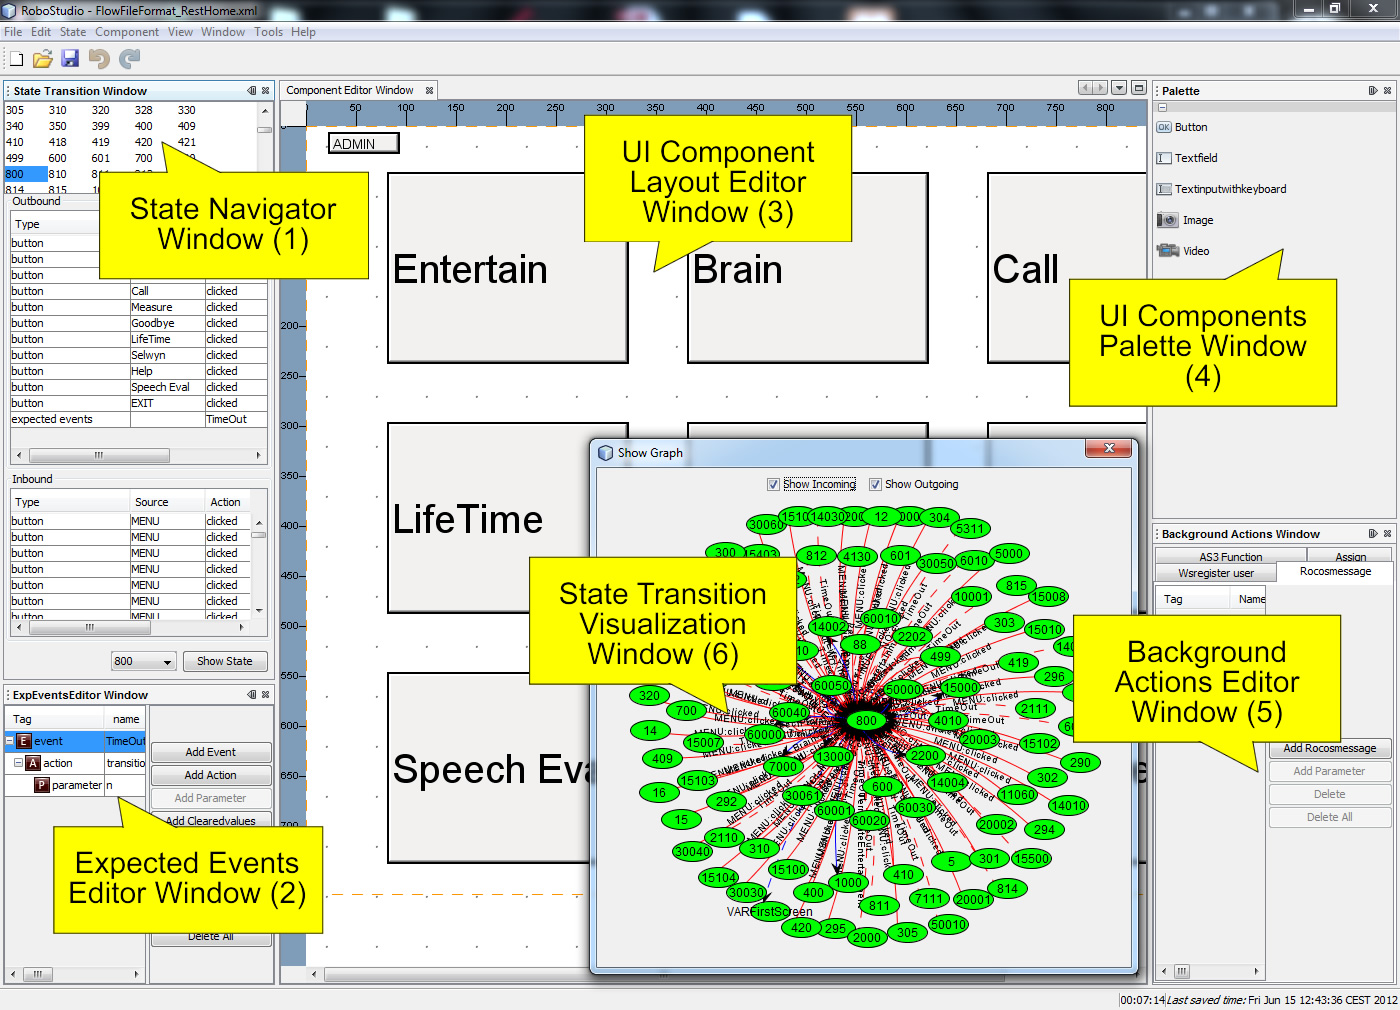
\includegraphics[width=\linewidth]{robostudio_vpe} 
  \caption{Window composition in Robostudio.}
  \label{fig:robostudio_vpe}
\end{figure}


%TODO: Vlt herausstellen, dass eine Schwierigkeit darin bestand, Verhaltensmodellierung und graphische Gestaltung unter einen Hut zu bringen (dazu Bild aus datta paper?). One challenge...






\section{Behaviour checking}
\label{sec:behaviourchecking}

The use of software is versatile from text editing programs running on personal computers, over control software for high-precision applications in aeronautics, right up to trigger mechanisms for deathly weapons. For most of them safety properties are irrelevant, but a few are ranked highly dangerous to their environment and also human lifes. In order to eliminate software malfunction there are different mathematical concepts for verifying software behaviour.
One of them is model checking wich allows checking state machine programs for functional safety. Since the healthbot applications mentioned in section~\ref{sec:healthbotapplication} are realised wth state machines, this concept of behaviour checking is applicable and important for our kind of programs. At first the basic idea of state machines is described in section~\ref{sec:statemachines}, followed by an intorduction into model checking in section~\ref{sec:modelcheckingandltl}.


\subsection{State machines}
\label{sec:statemachines}

A state machine is a model which can describe the behaviour of a system. It contains an aggregation of all different statuses of a system and possible changeovers from one status to another.

Each system status is represented by one \emph{state} which stands for a particular and unique constellation of system variables and properties. One state can be declared as \emph{start state} which is the very first state when the system starts working. The state representing the current system status is called \emph{current state}.
The current state changes whenever there is a modification to the system. Such transfers of the system from the current state to another one are defined by \emph{transitions}. Thus, they define the possible system behaviour.
All influences of the environment which cause a change to the system are called \emph{events}. They trigger transitions which transfer the system into a new state (current state). The fact that a state machine reacts to events is the reason why state machines are also called \emph{reactive systems}.

State machines can be visualized, as shown in figure~\ref{fig:statemachine} which gives a small example of a state machine.
\begin{figure}[htbp]
  \centering
  \tikzstyle{state} = [circle,fill=white,draw]
  \tikzstyle{stateblack} = [circle,fill=black!100,draw]
  \tikzstyle{every path} = [font=\sffamily\small]
  
	\begin{tikzpicture}[->,>=stealth',shorten >=1pt,auto,node distance=25mm]
	  \node[state] (1) {state 1};
	  \node[state] (2) [below right of=1] {state 2};
	  \node[state] (3) [above right of=2] {state 3};
	  \node[stateblack] (4) [above of=1,node distance=17mm] {};
	  
	  \path[]
	  	(1) edge [bend right] node [left] {event b} (2)
	        edge [bend left] node [above] {event a} (3)
	    (2) edge [bend right] node [right] {event d} (3)
	    (3) edge [bend left] node [above] {event c} (1)
	        edge [loop right] node {event e} (3)
	    (4) edge [right] node [right] {} (1)
	    ;
	\end{tikzpicture}
  \caption{General example for a state machine.}
  \label{fig:statemachine}
\end{figure}
All states are drawn as circles which contain their names. Transitions are painted as arrows between source and destination states, and the regarding trigger event names are written next to it.

The following example clarifies the concept of state machines. Assuming a door which can be opened, closed and locked by a key-operated bolt lock, the behaviour can be reduced to a state machine as shown in figure~\ref{fig:doorstatemachine}.
\begin{figure}[htbp]
  \centering
  \tikzstyle{state} = [circle,fill=white,draw]
  \tikzstyle{stateblack} = [circle,fill=black!100,draw]
  \tikzstyle{every path} = [font=\sffamily\small]
  
	\begin{tikzpicture}[->,>=stealth',shorten >=1pt,auto,node distance=35mm]
	  \node[state] (1) {closed};
	  \node[state] (2) [below of=1] {locked};
	  \node[state] (3) [right of=1] {opened};
	  \node[state] (4) [below of=3] {blocked};
	  \node[stateblack] (5) [left of=1,node distance=16mm] {};
	  
	  \path[]
	  	(1) edge [bend left] node [above] {open door} (3)
	        edge [bend left] node [above right] {turn key} (2)
	    (2) edge [bend left] node [left] {turn key} (1)
	    (3) edge [bend left] node [above] {close door} (1)
	        edge [bend left] node [right] {turn key} (4)
	    (4) edge [bend left] node [below left] {turn key} (3)
	    (5) edge [right] node [right] {} (1)    
	    ;
	\end{tikzpicture}
  \caption{Door behaviour as a state machine.}
  \label{fig:doorstatemachine}
\end{figure}
Four states represent the ``system statuses'' of a lockable door: closed but unlocked (closed), opened and unlocked (opened), closed and locked (locked), opened but locked (blocked). The latter case is when the extended bolt prevents the door from being closed.

The black dot defines the point of entry for this state machine, the door is closed but unlocked in the beginning. Through an event of the environment - in this case a human acting at the door - the door can be opened ,what makes ``opened'' the current state, and later be closed again. A turn of the key locks respectively blocks the door and no further opening or closing is possible. A second turn of the key un(b)locks the door again.

The short description given in this section does not contain a complete explanation about the concept of statemachines at all, but it gives a basic overview which is needed as background information for this work. Also the formal definition of state machines is not relevant and can be read in other literature~\cite{statemachines, statemachinesandformalmethods}.

%mathematical model of computation
%finite (endliche anzahl zust�nde)




\subsection{Model checking \& LTL}
\label{sec:modelcheckingandltl}

Whenever a software or hardware system has a special requirement in robustness and reliability, different formal methods are available to be used in order to verify the design.
Model checking is such a method which allows automatically verifying a system description against a specification by means of an exhaustive search of all states which could possibly be visited by the system during its execution. As a result, either the system description fulfills all propositions or a counter example is provided which gives evidence about a broken property. Figure~\ref{fig:modelchecking} gives a schematic view about the concept of model checking.

\begin{figure}[htbp]
  \centering
  \tikzstyle{state} = [circle,fill=white,draw]
  \tikzstyle{stateblack} = [circle,fill=black!100,draw]
  \tikzstyle{every path} = [font=\sffamily\small]
  \definecolor{egg}{RGB}{252,253,206}
  
	\begin{tikzpicture}[->,>=stealth',shorten >=1pt,auto,node distance=30mm]
	  
		\node[cloud, cloud puffs=15.7, cloud ignores aspect, align=center, draw, fill=egg] (model) at (0,5) {\parbox{2cm}{\centering system\\model}};
		
		\node[ellipse, draw, fill=egg] (properties) at (5,5) {\parbox{2cm}{\centering system\\properties}};
		
		\node[rectangle, draw, minimum width=2cm, minimum height=2cm, fill=egg] (checker) at (2.5,3) {\parbox{2cm}{\centering model\\checker}};
		
		\node[state, minimum width=2cm, minimum height=2cm,fill=red!40] (no) at (0,0) {\parbox{1.3cm}{\centering counter\\example}};
		
		\node[state, minimum width=2cm, minimum height=2cm,fill=green!40] (yes) at (5,0) {};
		
		\path[]
	  	(model)      edge [bend right] node {} (checker)
	    (properties) edge [bend left]  node {} (checker)
	    (checker)    edge [bend left]  node [above left] {not satisfied} (no)
	    						 edge [bend right] node [above right] {satisfied} (yes)
	    ;
		
	\end{tikzpicture}
  \caption{Concept of model checking.}
  \label{fig:modelchecking}
\end{figure}

For representing the system description - which can be a computer program, for example - a formal language is used. Also state machines are applicable to serve as a formal system description. In contrast, the specification used for model checking contains certain properties that express the desired and safe system behaviour in form of mathematical formulas. Linear temporal logic (LTL) is an example for a logic that is used to define such formulas on state machines. It is a temporal logic which can express formulas concerning the future of paths, for example, that something will eventually happen.

LTL is based on propositional logic, thus, it can express propositional variables ($p_1$, $p_2$, ...) and logical connectives ($\wedge$, $\vee$, $\neg$, $\rightarrow$ and $\leftrightarrow$). Additionally further temporal modal operators are provided which enable propositions concerning the future of paths, among three unary operators:

\begin{description}
	\item[$\Box \varphi$] This formula expresses that $\varphi$ is true now and in all following states. The meaning of the rectangle is ``GLOBALLY''.
	\item[$\medcircle \varphi$] With a circle representing ``NEXT'', $\varphi$ will be true in the next state.
	\item[$\Diamond \varphi$] At least one time - now or eventually in a later state - $\varphi$ is or will be true. The diamond stands for ``FUTURE''.
\end{description}

Furthermore, LTL provides binary operators as follows:

\begin{description}
	\item[$\varphi \mathcal{U} \psi$] The ``UNTIL'' operator makes $\varphi$ true until the first occurrence of a state where $\psi$ is true. Besides, $\psi$ will eventually be true.
	\item[$\varphi \mathcal{R} \psi$] It expresses that $\psi$ is true through the first occurrence of a state where $\varphi$ is true. Its meaning is $\varphi$ ``RELEASES'' $\psi$.
	\item[$\varphi \mathcal{W} \psi$] ``WEAK UNTIL'' represents the same as ``UNTIL'', except that an occurrence of $\psi$	is not necessary. In this case, $\varphi$ is true infinetely.
\end{description}

%Verkn�pfung von operatoren?






\section{Related work}
\label{sec:relatedwork}

%Was gibt es schon alles?

% 1993 A Visual-Programming Environment for a Temporal Logic Language
% 1995 Visual Specification of Branching Time Temporal Logic
% 2007 HomeTL: A visual formalism, based on temporal logic, for the design of home based care
% 2007 A Visual Editor to Support the Use of Temporal Logic for ADL Monitoring

%aim for simplifying the development of constraints, but they still demand knowledge of the underlying mathematical formalism of temporal logic.

The idea of a visual environment for the defining of system properties is not new and already pursued by some researchers. Although their focus does not completely match the subject of safety for healthcare robots, they present concepts of visualisation which might be relevant
% can be quite interesting 
for this work.
In section~\ref{sec:sisiruca}, the work of Sisiruc� and Ionescu is presented. Section~\ref{sec:delbimbo} dexcribes a three dimensional concept by Del Bimbo et al., followed by an introduction of HomeTL in section~\ref{sec:hometl}.

\subsection{Sisiruc� and Ionescu}
\label{sec:sisiruca}

A first step towards a graphical tool for designing safety constraints is taken by Sisiruc� and Ionescu~\cite{332301}. They developed an object-oriented graphical environment for visually creating temporal logic sentences and rules.
As shown in figure~\ref{fig:sisirucaandionescu}, the tool presents all operators as blocks which have inputs and outputs. 
\begin{figure}[htbp]
  \centering
  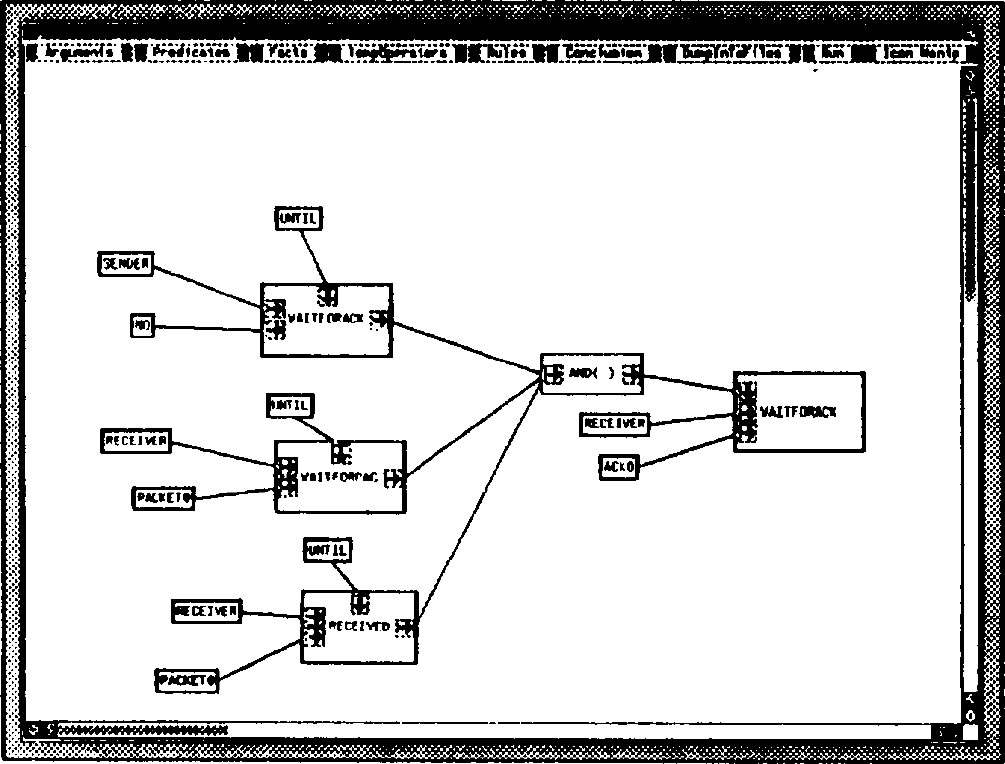
\includegraphics[width=0.6\linewidth]{sisirucaandionescu} 
  \caption{The visual programming environment. An example showing the ruel construction process~\cite{332301}.}
  \label{fig:sisirucaandionescu}
\end{figure}
Whereas logical operators such as \emph{AND} and \emph{OR} have their boolean output and inputs represented by arrows pointing to the right, generic blocks for temporal expressions additionally have an input symbolized by an arrow pointing downward where the temporal operator itself is to be attached. By adding and connecting the operators a big expression graph can be built. In case that a diagram becomes too complex, an implode feature allows to compress the graph to a single box. It is also applicable for the reuse of diagrams.

The presented environment aims to be an effective tool for developing temporal logic sentences and rules. In fact, it gives a schematic overview of even complex formulas and allows substitution and reuse. The visual formalism is an alienation of LTL which might be suitable for researchers, but probably not for novices.

%The tool presents temporal operators as logical modules with boolean inputs and outputs which can be connected to one big expression graph.



\subsection{Del Bimbo et al. (3D)}
\label{sec:delbimbo}

Del Bimbo and his colleagues worked on a visual tool for temporal logic, too, but with a special focus on hierarchical representation of formulas~\cite{520786}.
It is based on computation tree logic (CTL) which is a branching-time logic with support for quantifiers. In contrast to LTL where properties are fulfilled by all possible paths, CTL expresses properties which depend on the future branching, for example, that at least one path is existend which has a particular property.
As indicated by figure~\ref{fig:delbimbo}, the visual tool provides all operators known from LTL 
%The visual tool provides visual operators as shown in figure~\ref{fig:delbimbo}.
\begin{figure}[htbp]
  \centering
  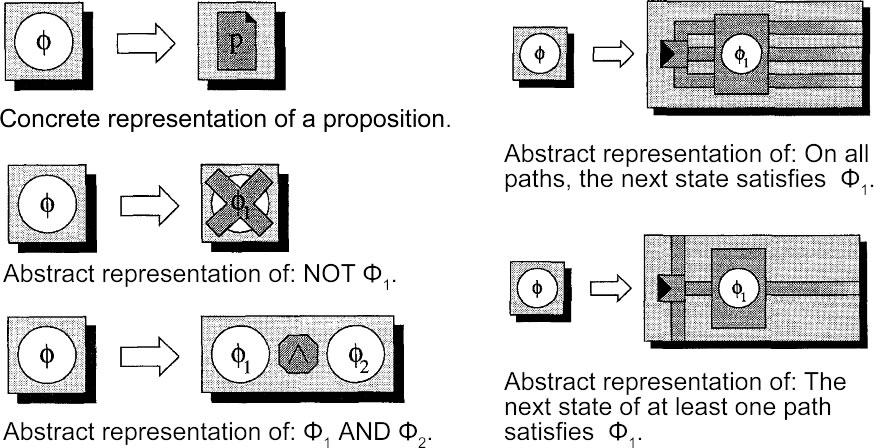
\includegraphics[width=0.8\linewidth]{delbimbo} 
  \caption{Some of the visual operators of Del Bimbo et al.~\cite{520786}.}
  \label{fig:delbimbo}
\end{figure}
except that temporal operators are extended by an existential or universal quantifier (``at least on one path...'', ``on all paths...'').


Except propositions all operators are abstract and have placeholders representing their subformulas which can be connected to other operators.
%Here each node of a tree is described by an abstract operator whose subformulas are represented by placeholders which can be connected to other operators.
The positioning of these operators is organized in layers where the parent operator lays one level above its children. It can be compared to a tree upside down with the topmost operator as root.
This formula structure can be visualized as a 3D branching tree within a virual space. Figure~\ref{fig:delbimbo3d} shows the result of considerations done by Del Bimbo and his colleagues.

\begin{figure}[htbp]
  \centering
  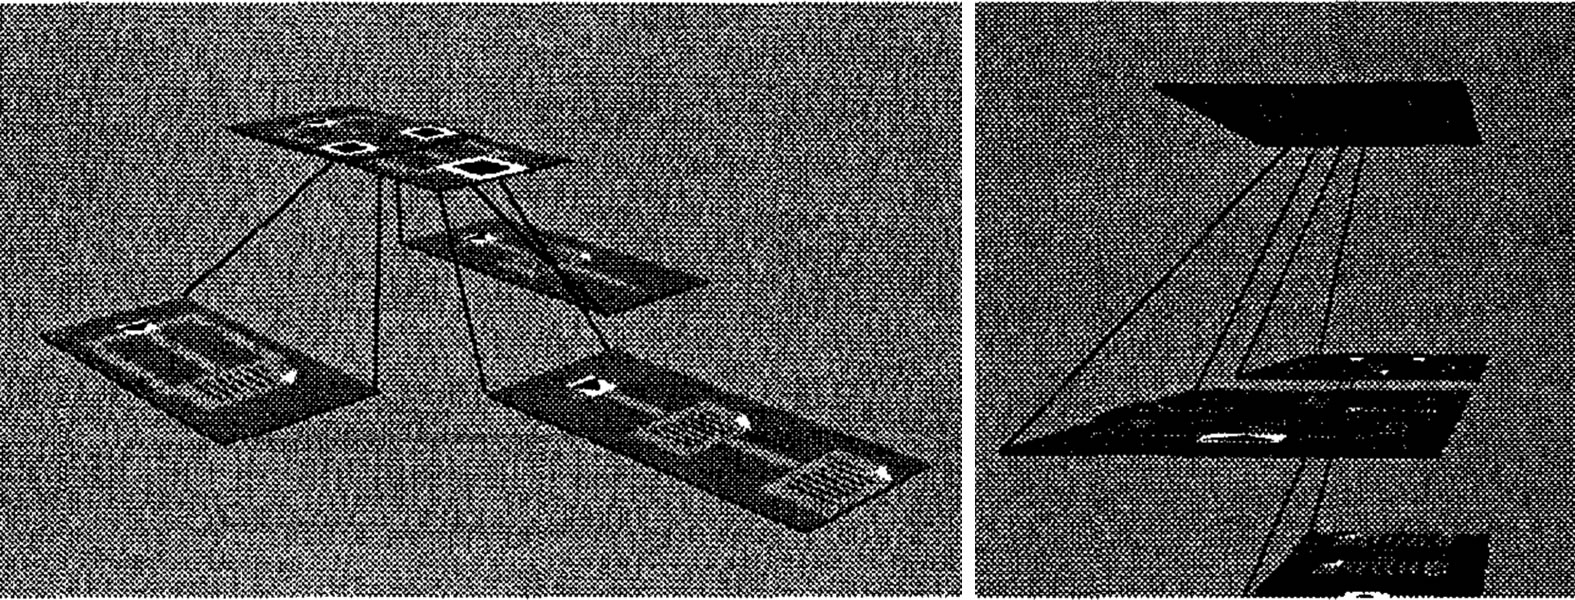
\includegraphics[width=1\linewidth]{delbimbo3d} 
  \caption{Formula trees' 3D representation within a virual space~\cite{520786}.}
  \label{fig:delbimbo3d}
\end{figure}

The presented visual formalism directly maps the syntax of the temporal logic onto graphic symbols and composition patterns. The researchers found well expressive graphical representations for all operator especially the temporal ones, what makes the tool fairly intuitive. The tree dimensional visualisation gives a good overview of the structure, although it shuld not be used for editing. Computer monitors can naturally display only two dimensions and input devices such as mouse and keyboard are customised to it. Editing of the third dimension needs special gesture definitions and 3D modelling techniques the most users might not be familiar with. Thus, a 3D representation for editing should only be used if necessary. This perception has been tried to be considered in this work.


%Die visualisierungen der Operatoren sind aussagekr�ftig, da sie Zukunft von Pfaden andeuten.
%A visual formalism has been presented which embeds the formal nucleus of this tool within a visual shell providing a one-to-one mapping of the syntax of the model onto graphic symbols and composition patterns.

%By exploiting 3D graphics, this visual representation breaks the native sequentiality of textual expressions and provides an explicit and intuitive representation for the three natural dimensions of branching time Temporal Formulae, i.e. time progression, parallelism among execution paths, and condition nesting.

%Both approaches are different fundamental ideas of representing temporal formulas. Whereas having a graph  seems not to be applicable for our approach, the idea of hierarchical operator representation of Del Bimbo et al. will be a good basis for our concept of constraint creation and understanding.



\subsection{HomeTL}
\label{sec:hometl}

The step towards a more abstract level of development is taken by HomeTL~\cite{4341725}, a visual formalism for the design of home based care. It allows healthcare professionals to specify rules and sequences of user actions in a quite nontechnical manner. Based on these conditions a monitoring system in a patient's home environment can detect and report abnormal situations within the daily routine.
The visual notation provides propositional variables and logical connectives, the latter is shown in figure~\ref{fig:hometloperators}. In contrast to LTL, the temporal operators of HomeTL use absolute time limits (seconds, for example) which are defined by $\tau$. Thus, not only the relative order of states is defined but also a time by which a particular action has to happen.

\begin{figure}[htbp]
  \centering
  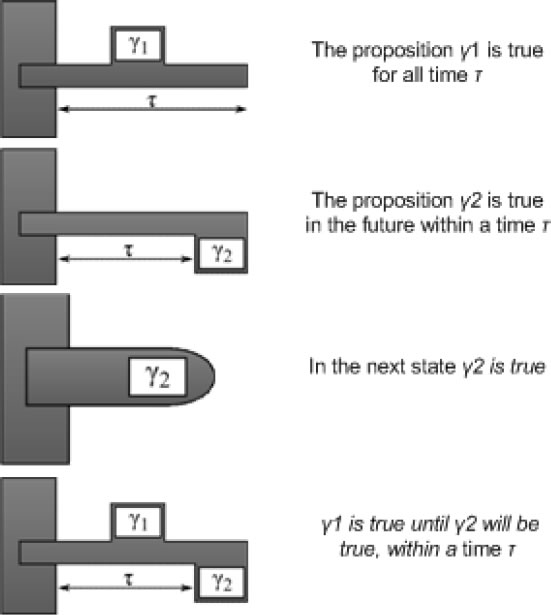
\includegraphics[width=0.5\linewidth]{hometloperators} 
  \caption{Graphical representation of visual notation for temporal
operators within HomeTL user interface~\cite{4341725}.}
  \label{fig:hometloperators}
\end{figure}

This notation uses special meanings for the two dimensions: The horizontal dimension shows the temporal evolution of states, while the vertical dimension expresses the logical relationships at the respective current state. A programming environment allows editing and creating of constraints by using the atomar operators. Figure~\ref{fig:hometleditor} presents a snapshot of this editor.

\begin{figure}[htbp]
  \centering
  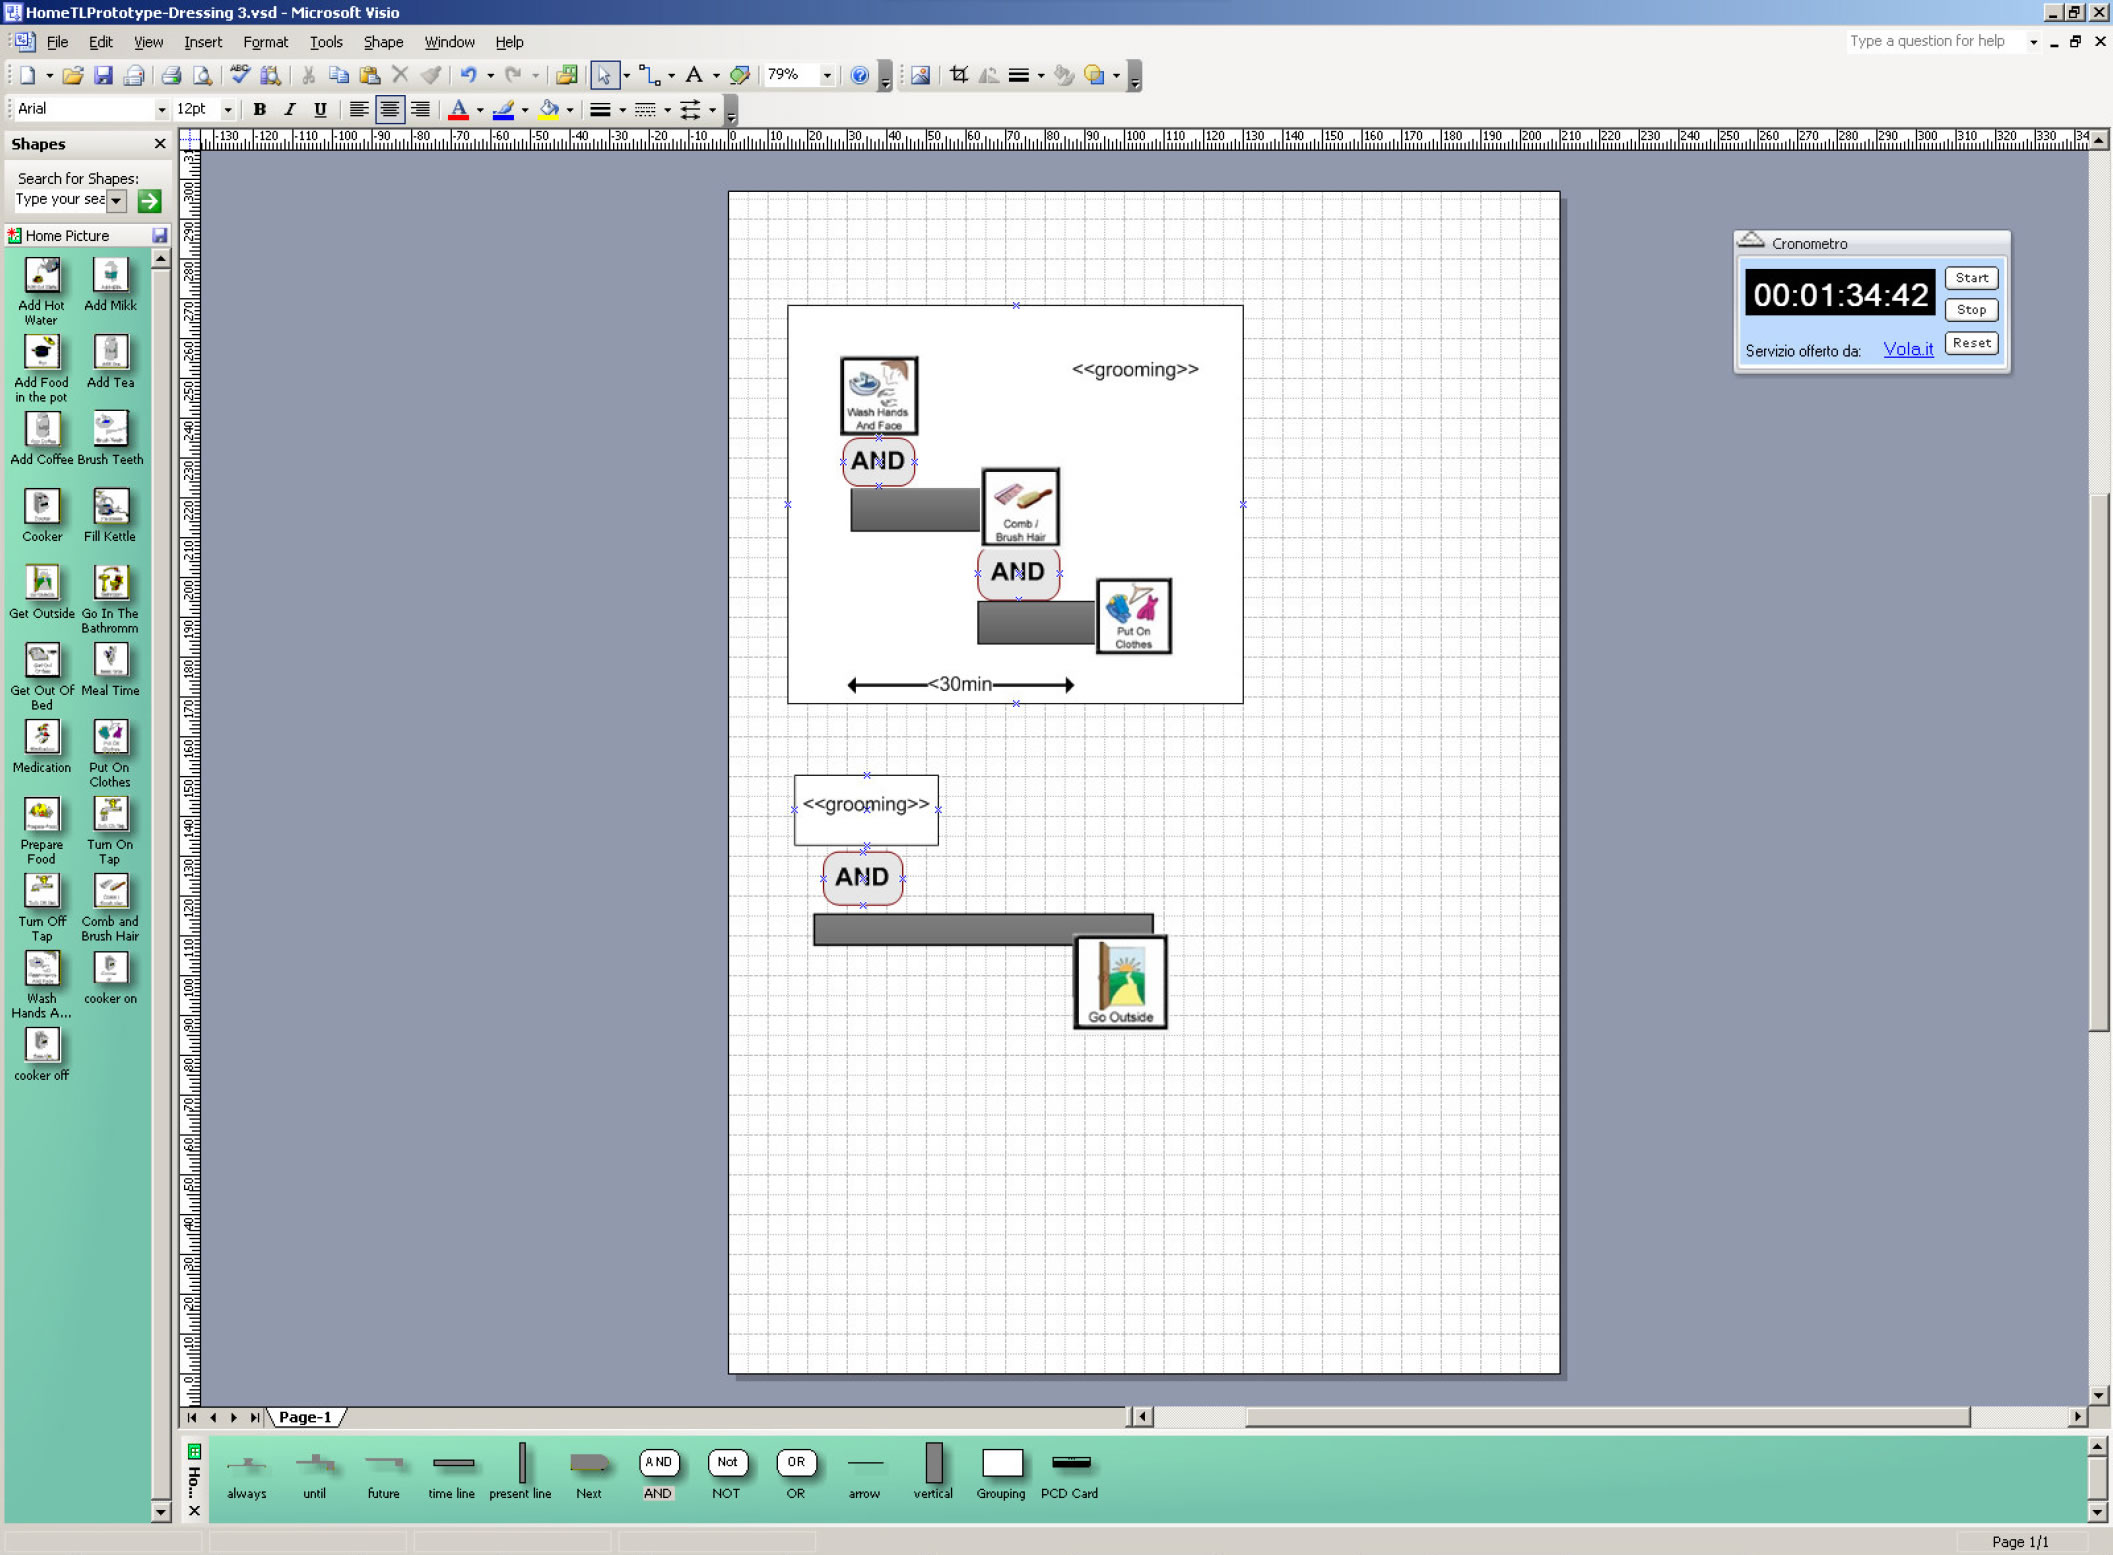
\includegraphics[width=\linewidth]{hometleditor} 
  \caption{HomeTL Visual Editor~\cite{4341725}.}
  \label{fig:hometleditor}
\end{figure}

Even though this approach touches the subject of healthcare it barely matches the problem stated in this work. HomeTL focuses more on monitoring temporal boundaries of a patient's behaviour than on ensuring functional safety of an implemented program. It does however depict how nontechnical constraint design can be realised and its graphical design is a good example of handling time dependencies.






%There are already works about constraint generation such as one approach of NASA [4], for example. They used test oracles in order to achieve consistency between program code and specification during development. 
% Das wollen wir auch erzielen mit unseren automatisch generierten constraints...
%But these kind of oracles are for automated test purpose and are rather complex than intuitive. However, our goal is to find nonmathematical and just intuitive ones. An intelligent heuristic must determine key states and possible conjunctions of them in order to build reasonable constraints. Afterwards they get filtered by an algorithm which computes importances for each constraint based on state weights. Finally the developer obtains a set of visual constraints which he can then check for plausibility.